\documentclass[11pt]{article}
\usepackage{mathptmx}

\usepackage{setspace}
\usepackage{amsmath,amssymb}
\usepackage{amsthm}
\usepackage{fancybox}
\usepackage{algorithm, algpseudocode}
\usepackage{url}

\usepackage[font=footnotesize]{caption}
\usepackage{multirow}
\usepackage{color}
\usepackage{graphicx}
\usepackage{setspace}
\usepackage{comment}
\usepackage{bm}
\usepackage{enumitem}
\usepackage{makecell}
\usepackage[breakable, theorems, skins]{tcolorbox}
\DeclareRobustCommand{\mybox}[2][gray!20]{%
\begin{tcolorbox}[   %% Adjust the following parameters at will.
        breakable,
        left=0pt,
        right=0pt,
        top=0pt,
        bottom=0pt,
        colback=#1,
        colframe=#1,
        width=\dimexpr\textwidth\relax, 
        enlarge left by=0mm,
        boxsep=5pt,
        arc=0pt,outer arc=0pt,
        ]
        #2
\end{tcolorbox}}

\newcommand*{\KeepStyleUnderBrace}[1]{%f
  \mathop{%
    \mathchoice
    {\underbrace{\displaystyle#1}}%
    {\underbrace{\textstyle#1}}%
    {\underbrace{\scriptstyle#1}}%
    {\underbrace{\scriptscriptstyle#1}}%
  }\limits
}



\usepackage[margin=1in]{geometry}
 
\allowdisplaybreaks[4]
\usepackage{bbm}


\usepackage{amsrefs}
\usepackage{mathtools}
\mathtoolsset{showonlyrefs=true}


\usepackage[utf8]{inputenc}
\usepackage{hyperref}
\hypersetup{
    colorlinks=true,
    citecolor = blue,
    linkcolor=blue,
    filecolor=magenta,           
    urlcolor=black,
}

\usepackage[breakable, theorems, skins]{tcolorbox}
\DeclareRobustCommand{\mybox}[2][gray!20]{%
\begin{tcolorbox}[   %% Adjust the following parameters at will.
        breakable,
        left=0pt,
        right=0pt,
        top=0pt,
        bottom=0pt,
        colback=#1,
        colframe=#1,
        width=\dimexpr\textwidth\relax, 
        enlarge left by=0mm,
        boxsep=5pt,
        arc=0pt,outer arc=0pt,
        ]
        #2
\end{tcolorbox}
}
\newtheoremstyle{exampstyle}
  {.3\topsep} % Space above
  {.1\topsep} % Space below
  {} % Body font
  {} % Indent amount
  {\bfseries} % Theorem head font
  {.} % Punctuation after theorem head
  {.5em} % Space after theorem head
  {} % Theorem head spec (can be left empty, meaning `normal')


\def\sign{\textup{sgn}}
\theoremstyle{exampstyle} 
%\theoremstyle{definition}
\newtheorem{thm}{Theorem}[section]
\newtheorem{lem}{Lemma}
\newtheorem{prop}{Proposition}
\newtheorem{pro}{Property}
\newtheorem{cor}{Corollary}[section]
\newtheorem{assumption}{Assumption}
\newtheorem{defn}{Definition}[section]
\newtheorem{example}{Example}[section]
\newtheorem{rmk}{Remark}
\usepackage{dsfont}

\theoremstyle{definition}
\newtheorem{open}[]{Open problem}

 \usepackage[parfill]{parskip}

\usepackage[compact]{titlesec}

\usepackage{sectsty}

\sectionfont{\fontsize{11.5}{10}\selectfont}
\subsectionfont{\fontsize{11}{10}\selectfont}
\usepackage[compact]{titlesec}
\titlespacing{\subsection}{0pt}{*0}{-4pt}
\titlespacing{\subsubsection}{0pt}{*0}{*0}


\usepackage{mathrsfs}
\newcommand{\SNR}{{\rm SNR}}
\def\sign{\textup{sgn}}
\def\srank{\textup{srank}}
\def\rank{\textup{rank}}
\def\caliP{\mathscr{P}_{\textup{sgn}}}
\def\caliF{\mathscr{F}_{\textup{sgn}}}


\usepackage{algpseudocode,algorithm}
\algnewcommand\algorithmicinput{\textbf{Input:}}
\algnewcommand\algorithmicoutput{\textbf{Output:}}
\algnewcommand\INPUT{\item[\algorithmicinput]}
\algnewcommand\OUTPUT{\item[\algorithmicoutput]}

\input macros.tex


\begin{document}
\begin{center}
{\bf \large High-dimensional Tensor Learning: The Good, the Bad, and the Pragmatic}\\
\vspace{.1cm}
Miaoyan Wang, July 2021
\end{center}
\vspace{-.5cm}
\section*{Overview}
\vspace{-.5cm}
High dimensional tensor methods are making enormous impacts on science and society. The empirical successes, however, are uncovering pressing new challenges that stand in the way of further progress: decisions arising from classical statistical premises are sensitive to model misspecification; greedy algorithms are yielding biased solutions; and concerns on prediction-interpretability balance continue to mount. 


These challenges can be addressed only by an appeal to a genuine combination of multidisplinary approaches. {\bf We propose to develop a suite of statistical learning theory, efficient algorithms, and data-driven solutions for high-dimensional tensor problems.} The research agenda spans the full spectrum of multilinear analysis tools in modeling, statistical-computational balance in estimation, and robust algorithms with accuracy guarantees. Unlike matrices, higher-order tensor problems are NP-hard in general. The PI's work will investigate the intrinsic low-dimensionality for a wide range of structured tensors including, but not limited to, low-rankness, non-negativity, block-structure, and smoothness. The new parametric and nonparametric framework for addressing higher-order high-dimensional tensor problems will provide solutions that were previously impossible. 

Tensor data analysis is an integral part of modern domain sciences. The new directions have been particularly motivated by three applications: the classification and comparison of brain connectivity data, the integration of omic (genome, transcriptome, proteome) data, and the pattern detection in social recommendation system. {\bf The developed tools will allow domain scientists to examine complex interactions among tensor entries and between multiple tensors, thereby providing solutions to questions that cannot be addressed by traditional analysis.} 

{\bf Intellectual Merit.} The proposal lays out an ambitious plan for a full spectrum of parametric, non-parametric, higher-order, high-dimensional tensors with multimodal data integration. 
The PI has an excellent record of pushing disciplinary boundaries by synthesizing knowledge and experience from diverse areas. The PI has a unique combination of post-graduate training in statistics (2010-2015), mathematics (2015-2017), computer science (2015-2018), and genomics (2013-2018). The proposed research builds on the PI's established high-impact tensor work ranging from theory~\cite{wang2018learning, han2020exact,wang7,wang8,wang2} to methodology~\cite{wang2019multiway, wang1, wang3, wang4, pmlr-v119-lee20i}) to domain science~\cite{wang2019three,wang5,wang9,wang6,wang10}. PI has established herself as an outstanding teacher-scholar in multiple disciplines, including two 2021 Best Student Paper Awards (mentored by the PI as advisor) from American Statistical Association, Charles J. Epstein Trainee Semifinalist Award from American Society of Human Genetics, and IGES Williams Finalist Award from International Genetic Epidemiology Society. The PI’s work has a transformational nature involving connections across diverse disciplines, and the PI strives to push the boundary of interdisciplinary research further.

{\bf Broader Impacts.} The PI will integrate the research and eduction goals by establishing a unique research-training experience, thereby broadening participation in STEM fields. Comprehensive plans for education and outreach will draw on PI's past success and leverage institutional resources through the four-university TRIPODS and Data Science Hub that the PI is affiliated with.
The PI will organize and host summer research positions that engage a diverse student body at all levels of seniority. New courses on {\it fairness in data science} will be created in both traditional and online formats. The course focuses on critical thinking skills and development of equitable access for underrepresented groups. The PI is committed to training students the interdisciplinary skills for them to make independent, insightful contributions to the larger society. Collaborations with domain science researchers in academia and non-profit labs will continue through the established channels. The research-training agenda is well integrated into the education, which as a whole, creates an inclusive environment for every student to succeed in their own individual careers.  
 
 
\newpage
\setcounter{page}{1}
\begin{center}
{\bf \large High-dimensional Tensor Learning: The Good, the Bad, and the Pragmatic}\\

Miaoyan Wang, UW-Madison
\end{center}
\vspace{-.3cm}

\section{Research Goals and Significance}
\vspace{-.5cm}
My proposed research is in the intersection of statistics, machine learning, and optimization, with a focus on tensor data analysis. Rapid developments in modern technologies have made multiway data readily available in daily lives. Tensor provides a generalized data structure in many learning procedures. Methods built on tensors provide powerful tools to capture complex structures that lower-order methods fail to exploit. The ambitious goal in my proposal is to create new horizons in tensor methods and applications across the disciplines of mathematics, computer science, and biomedical sciences.  

\setlength{\abovedisplayskip}{6.5pt}
\setlength{\belowdisplayskip}{6pt}


Below I give two examples of biomedical tensor data arising from my current collaborations. I will propose the core fundamental challenges based on the questions raised in the applied endeavors.

{\bf Multi-tissue, multi-individual gene expression.} The recent completion of Genotype-Tissue Expression (GTEx, Figure~\ref{fig:intro}a) project has provided an unprecedented opportunity to investigate transcriptome diversity and complexity. A typical multi-tissue experiment collects gene expression profiles from different individuals in a number of tissues.  The study results in a huge compendium of tensor data consisting of millions of expression measurements from over 20K genes across 544 individuals and 53 human tissues. My previous work~\cite{wang2019three} reveals that the variation in the expression levels is attributable to genes, tissues, individuals, and interactions thereof. Understanding the multiway patterns of whole-genome transcriptome variation is crucial to unravel unravel genomic basis for tissue functions and personalized medicines.

{\bf Multimodal neuroimaging data analysis.} The Human Connectome Project (HCP, Figure~\ref{fig:intro}b) consists of massive datasets representing the anatomical and functional connectivities across brain regions from over 1,200 individuals. Multimodal brain connectivity networks are constructed based on various measurements, including functional magnetic resonance imaging, electroencephalography, and diffusion tensor imaging. My previous work~\cite{wang2018learning,pmlr-v119-lee20i} provides strong evidence for inter- and intra-modal correlation in the brain network data. Efficient multiway methods are essential for further investigating the structural and functional connectivities in human brains. 
\begin{figure}[http]
\begin{center}
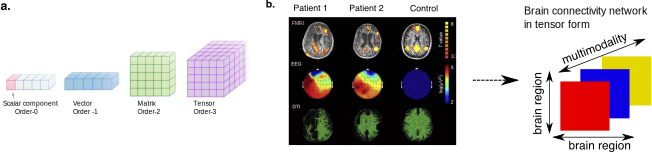
\includegraphics[width=1\textwidth]{example.pdf}
\vspace{-.8cm}
\caption{(a) GTEx collects gene expression profiles of over 20,000 genes from 544 individuals across 53 human tissues. (b) HCP collects multimodal imaging data from over 1,200 individuals. Figures are reproduced based on~\cite{timpson2018genetic, bruno2011multimodal}.}\label{fig:intro}
\vspace{-.6cm}
\end{center}
\end{figure} 

In the above two examples and many other applications, scientists are interested in identifying interpretable latent structure within the high-dimensional tensor data. The research question goes beyond the traditional multivariate analysis: we are interested in the distribution over multi-indexed entries in order to capture the multilinear relations among variables. Recent years have seen an upsurge of interest in tensor data analysis. However, the empirical success has uncovered a myriad of new and pressing challenges. Multidisciplinary efforts are necessary to address these challenges.

\begin{itemize}[wide,labelwidth=!, labelindent=0pt,itemsep=0ex,parsep=0ex,topsep=-3pt]
\item {\bf Old premises fail in new settings.} High-dimensional tensor models and multilinear algorithms can yield unexpected behaviors that challenge classical statistical premises. Notable examples include {\it double descent} (i.e., no bias-variance trade-off in overparameterized tensor models~\cite{NEURIPS2020_f9d3a954, belkin2019reconciling}) and \emph{benign non-convexity} (no spurious local optima in tensor factorization~\cite{ge2020optimization}). Classical statistical premised need be revolutionized to address the potential and limitations of new settings. 
\item {\bf Multiple complexity measures interact.} Complexity is the fundamental tool in modern data science to characterize the difficulty of learning tasks. Statistics use {\it model complexity} to measures the number of samples needed for accurate estimation. Computer sciences use {\it computational complexity} to measure the number of arithmetic operations required in optimization algorithms. The fundamental challenges of tensor problems lie in the computational-statistical tradeoffs, in which model complexity hinges on and interacts with computational complexity. Current mechanisms for optimizing these tradeoffs are limited.
\item {\bf One paradigm may not fit all.} Off-the-shelf tensor data analytics tools are increasingly challenged by important domain applications~\cite{murdoch2019definitions}. Parametric model facilitates statistical inference but often lacks the robustness; nonparametric model boosts the prediction but hinders the interpretation; classical asymptotic theory holds only for exponential time algorithms but is brittle with computational constraints. In these practical situations, we need to carve out the regimes for which a learning approach succeeds and/or fails. Challenges associated with ever-growing tensor applications await breakthroughs in understanding. 
\end{itemize}

 {\bf The proposed project is to develop a suite of statistical learning theory, efficient algorithms, and data-driven solutions for high-dimensional tensor problems.} The developed tools will allow domain scientists to examine complex interactions among tensor entries and between multiple tensors, thereby providing solutions to questions that cannot be addressed by traditional analysis.  The detailed plan of my research agenda is organized into three core themes: 
 
{\bf  Aim 1.\ Parametric tensor models with statistical and computational optimality.} Block tensors arise frequently in neuroimaging, recommendation system, topic modeling, and sensor network localization. Despite the popularity, little is known about the fundamental limits in tensor block models. The block tensor serves as a meta structure to most---if not all---common models including the low-rankness~\cite{young2018universality}, latent space models~\cite{wang2018learning}, and isotonic tensors~\cite{pananjady2020isotonic}. We plan to use tensor block models as a lens to explore statistical and computational trade-off in parametric structured tensor problems. We will fully characterize, for the first time, the critical signal-to-noise threshold in block tensor models, revealing the intrinsic distinctions between (vector) clustering, (matrix) biclustering, and (tensor) higher-order clustering. The results generalize existing low-rank methods and provide solutions that were previously impossible. See Section~\ref{sec:theme1}.

{\bf Aim 2.\ Beyond low-rankness:\ nonparametric estimation and completion for high-rank tensors.} Parametric tensor models (e.g.,\ low-rank models, block models) aim to explain data with a finite number of parameters; these methods are useful when the sample outsizes the parameters. Nonparametric models, on the other hand, use infinite number of parameters to allow growing model complexity as sample increases. In this vein, we aim to develop nonparametric tensor models to effectively address both low- and high-rank structures. We will develop a new complexity framework to capture nonlinear high-rank signals, while encompassing existing models---including CP models~\cite{kolda2009tensor}, Tucker models~\cite{de2000multilinear}, single index models~\cite{ganti2015matrix}---as special cases. The approach leads to a substantially richer class of tensor models in many learning problems, including regression, completion, multi-task learning, and compressed sensing. See Section~\ref{sec:theme2}.

{\bf Aim 3.\ Predictive tensor models with auxiliary information.}
Predictive learning models are useful in daily decision making tasks, i.e.,\ predicting diseases based on multimodal neuroimaging, classifying documents based on their contents, and deciding target customers based on shopping behaviors in recommendation system. These problems are often formulated as predicting the response variable $Y_{\text{new}}$ from explanatory variable $X_{\text{new}}$, where the sample available is in the form of pairs $(X_i, Y_i)_{i=1,\ldots,n}$. We plan to combine tensor structure models with predictive tasks, by jointly estimating the latent structure in tensors as well as the relationship between the tensor data and auxiliary features. The outlined direction builds new links between machine learning methodology and scientific discovery, and also produces new areas in which machine learning theory and applications complement each other. See Section~\ref{sec:theme3}. 

{\bf PI's qualification and prior supports}. The PI is a young faculty member in the Department of Statistics at UW-Madison. The PI is also affiliated with Institute for Foundations of Data Science (IFDS), an NSF-funded TRIPOD Phase II collaboration initiative between four universities. The PI has an excellent track record and a unique combination of training background in mathematics (2006-2010), statistics (2010-2015), genetics (2015-2018), and computer science (2015-2018). The PI's current work is supported by NSF MDS-1915978 ``spectral methods for high dimensional tensor data'' (Sep 2019 - Aug 2022, \$179,349 in total). 

The PI has built tremendous momentum since the tenure track position. The PI is prolific in publishing papers in top methodological venues (NeurIPS, ICML, etc~\cite{wang2019multiway, wang1, wang3, wang4, pmlr-v119-lee20i}), applied venues (PNAS, AOAS, etc~\cite{wang2019three,wang5,wang9,wang6,wang10}), and theory venues (JMLR, AOS, etc~\cite{wang2018learning, han2020exact,wang7,wang8,wang2}). Most of these publications are exclusively with PI's students; this has demonstrated the independence and leadership of PI in research and education. The past NSF grant has supported the PI and the students to deliver over 40 talks at departmental seminars in the US, Canada, and Europe, as well as invited talks at international conferences including JMS, AMS, ENAR, IMS, and SIAM. The PI's research group has developed 15 open-source software packages in R, Matlab, and C. All packages are regularly maintained on CRAN and Github. 

As a young female faculty member, the PI has demonstrated effective integration of research and education. The PI is leading a diverse research group, and has served as co-advisor/committee for students in Statistics, Industrial Engineering, and Civil Engineering. The PI has won {\bf two Best Student Paper Awards (with PI as the advisor)} from American Statistical Association in 2021, the Madison Teaching and Learning Excellence Fellow, and multiple prestigious young researcher awards in statistics, machine learning, and genetics.  A highlight of the PI's achievement is to engage undergraduate students from underrepresented population into cutting-edge research; these projects have resulted in publications at NeurIPS (the best venue in machine learning). The PI's research/eduction integration has attached media coverage and been featured in the online article \emph{``Women in STEM: 5 Thoughtful Ways to Recruit and Retain Them''}~\cite{wang11}. 

The agenda in this proposal has broader impacts on multiple research fields and education. The PI’s work has a transformational nature involving connections across diverse disciplines, and the PI strives to create a welcoming venue for diverse trainees, thereby broadening participation in STEM. The proposal lays out an ambitious plan for a full spectrum of parametric, non-parametric, high-rank, high-dimensional tensors with multimodal data integration. Education and research will be integrated in the form of developing new courses, creating summer research-training positions, and engaging underrepresented students in outreach. Theory and application will be combined with the emphasize on data-intensive problems in social network science and biomedical science. More detailed plan will be described in Section~\ref{sec:impact}. 


\section{AIM 1.\ Parametric Tensor Models with Statistical and Computational Optimality}\label{sec:theme1}
\vspace{-.4cm}

\mybox[gray!20]{
This section focuses on unsupervised clustering methods for high-dimensional tensors, where the learner has little or no label information during training. The modeling is notably difficult due to limited information. The proposed research provides tools for optimizing trade-off between statistical and computational efficiency in parametric tensor models.}

We focus on tensors of order 3 or greater, known as higher-order tensors. A tensor $\Theta \in  \mathbb{R}^{d_1 \times\cdots \times d_K}$ is a higher-order generalization of matrix that obeys the mode-$k$ multiplication rule~\cite{kolda2009tensor} denoted by $\times_k$: $\Theta\mapsto \Theta\times_1\mM_1\times_2\cdots\times_K\mM_K$, for matrices $\mM_k$ of consistent dimensions. Higher-order tensors are not simply matrices with more indices; rather, they are data objects whose structures remain covariant under multilinear transformations. Key challenges of multilinear nonconvesity await breakthroughs in understanding. 

\vspace{-.5cm}
\subsection{Motivation}
\vspace{-.3cm}
A central theme in modern data analysis is to find a low-dimensional representation to better understand, compress, and convey the key phenomena buried in noisy observations. Dimension reduction is crucial for large-scale tensor data analysis. The most popular model in tensor dimension reduction is the multilinear low-rank model. An order-$K$ $(d_1,\ldots,d_K)$-dimensional tensor $\Theta$ is called Tucker low-rank if it can be represented by some low-dimensional core tensor $\tS$ under a change of basis
\begin{equation}\label{eq:Tucker-low-rank}
\Theta = \tS \times_1 \mM_1 \times_2 \cdots \times_K \mM_K
\vspace{-.2cm}
\end{equation}
for some transformation matrices $\mM_k\in\mathbb{R}^{d_k\times r_k}$ with $r_k\ll d_k$ along each of the modes (see Figure~\ref{fig:1}c).  

Low-rank formulation has been actively studied in various contexts, such as tensor regression \cite{zhou2013tensor,wang4}, tensor completion \cite{pmlr-v119-lee20i,gandy2011tensor}, tensor PCA \cite{zhang2018tensor,wang7}, and generalized tensor learning \cite{han2020optimal}. A special but more fundamental low-rank model, \emph{multiway tensor block model}, however has yet to be investigated. In comparison with general low-rankness, the discrete block structure provides better interpretation, because the transformation matrix $\mM_k$ encodes the clustering membership along the mode $k$ of the tensor. Figure~\ref{fig:1}a shows an order-3 tensor with a block structure, in which each of the modes is partitioned into several clusters. The goal is to identify the block structure, as well as to recover the true signal tensor, from a noisy observation. The tensor block model and higher-order clustering arise commonly in practical applications. For example, 

\begin{itemize}[wide, labelwidth=!, labelindent=0pt,topsep=-7pt]
\item \emph{Multi-tissue Gene Expression Analysis.} Gene expression profiles such as scRNA-seq and microarrays are collected from multiple individuals across numbers of tissues~\cite{mele2015human,wang2019three}. Genes involved in the same biological function exhibit similar expressions within a group of tissues and individuals, while these expression values vary from group to group. Similarly, tissues and individuals exhibit gene-specific clustering patterns. Identifying complex interactions among these three entities is of great interest to biomedical research. 

 \begin{figure}[http]
\begin{center}
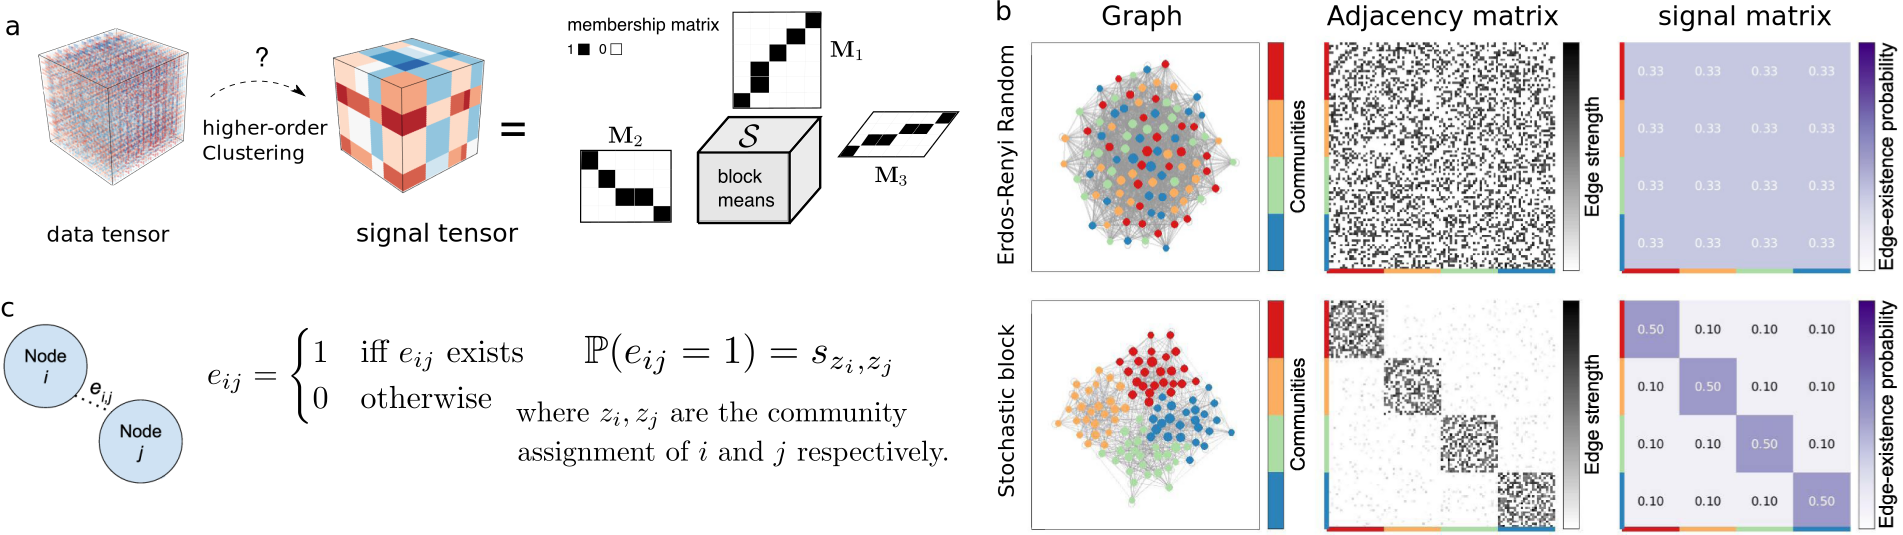
\includegraphics[width=1\textwidth]{network1.pdf}
\caption{(a) Tensor block model generalizes usual matrix block model and is useful for higher-order clustering~\cite{han2020exact}. (b) Examples of common social connectivity networks~\cite{faskowitz2018weighted}. (c) Representation of connectivity edges in the usual stochastic (matrix) block model.}\label{fig:1}
\end{center}
\vspace{-.2cm}
\end{figure}
   
\item \emph{Multilayer Network Analysis.} A multi-layer network consists of multiple undirected graphs (or adjacency matrices), where each graph represents the connection among the same set of vertices (Fig~\ref{fig:1}b-c). The data structure is naturally organized as an order-3 tensor with the first two modes being vertices and the third mode being the contexts under which the graph is observed. Multilayer networks arise commonly in longitudinal study of network~\cite{lei2019consistentcommunity} and multi-relational data~\cite{wang3, wang4}. While the community structure in single-layer network has been widely analyzed in the literature, little work has studied the heterogeneous pattern across multiple layers. The connectivity within/between communities may change correspondingly as the context changes, and it is important to simultaneously obtain the clusters across different contexts. 
    
\item \emph{Online Click-through Prediction.} In e-commerce, predicting click-through for user-item pairs in a time-specific way plays an important role in online recommendation system~\cite{sun2015provable}. The click-through data can be organized as an order-3 tensor, where each entry indexed by (users, items, time) represents the presence or absence of user-item action across 24 hours in a day. The users and items often exhibit clustering structures due to user features and item attributes, respectively. The shopping behavior also varies in time, and this heterogeneity depends on the specific groups of users and items. For instance, salarymen tend to have higher activities than non-office workers in the period of after-work hours. 
\end{itemize}


%\vspace{-.1cm}
\subsection{Multiway Tensor Block Models}
\vspace{-.2cm}
Methods built on tensors provide generalized tools to capture complex data structure. For cleaner illustration, we consider balanced setting with equal dimension and cluster size in each of the tensor modes. Let $\tY\in\mathbb{R}^{d\times \cdots \times d}$ be an order-$K$ data tensor of interest. The main assumption of tensor block model is that the observed data tensor $\tY$ is a noisy realization of a signal tensor that exhibits a checkerbox structure (see Figure~\ref{fig:1}a). Specifically, suppose there are $r$ clusters on each of the $K$ modes, and we represent the clustering along the model $k$ by a vector $\mz_k =(z_{k,1},\ldots, z_{k,d})^T\in [r]^{d}$, for all $k\in[K]$. Under the block structure, the entries $\tY(i_1,\ldots,i_d)$ are realizations from the model
\begin{equation}\label{eq:model-tensor-entry}
\tY(i_1,\ldots,i_K)=\tS(z_{1,i_1},\ldots,z_{K,i_K})+\tE(i_1,\ldots,i_K),\quad \text{for all } (i_1,\ldots,i_K)\in[d]^K,
\end{equation}
where $\tS\in\mathbb{R}^{r\times \cdots\times r}$ is a low-dimensional core tensor, and $\tE$ is a noise tensor consisting of i.i.d.\ zero-mean Gaussian entries with variance $\sigma^2$. Model~\eqref{eq:model-tensor-entry} can be equivalently written in tensor-matrix product: 
\begin{equation}\label{eq:model-tensor}
\tY = \tS \times_1 \mM_1 \times \cdots \times_K \mM_K + \tE,
\end{equation}
where $\mM_k \in \{0,1\}^{d\times r}$ is the membership matrix associated with $\mz_k$ such that $\mM_k(i,j) = 1$ if and only if $z_{k,i} = j$. That is, $\mM_k$ has one copy of 1 and $(r-1)$ copies of 0's in each of the rows. We use forms \eqref{eq:model-tensor-entry} and \eqref{eq:model-tensor} exchangeably for notational convenience. 

The learning goal is to estimate multiway connection signal $\tS$ and clustering assignments $\mM_k$ from a noisy observation $\tY$. We focus on two inference tasks for tensor block model:
\mybox[gray!20]{
\begin{open}
\begin{itemize}[leftmargin=*]\hfill
\item (Clustering) How to recover the membership matrices $\mM_k$, or equivalently the label vectors $\mz_k$?
\item (Denoising) How to accurately estimate the underlying signal tensor $\tS$?
\end{itemize}
\end{open}
}


\vspace{-.2cm}
\subsection{Proposed Agenda: Statistical and Computational Phase Transition}
\vspace{-.2cm}
My initial investigation reveals a surprising but simple characterization for the models~\eqref{eq:model-tensor-entry} and~\eqref{eq:model-tensor}. 
\begin{defn}[A key quantity for hardness of the problem]
The statistical and computational hardness of tensor block model is completely determined by the following signal-to-noise ratio (SNR),
\[
\SNR= \Delta_{\min}^2/\sigma^2,\quad \text{~where } \Delta_{\min}^2 := \min_{k\in [K]}\min_{j_1 \neq j_2} \FnormSize{}{\text{Unfold}_k(\tS)_{j_1:} - \text{Unfold}_k(\tS)_{j_2:}}^2,
\]
where $\text{Unfold}_k(\tS)_{j:}$ denotes the $j$-th row of the matrix obtained by unfolding the tensor $\tS$ along mode $k$. 
\end{defn}
We aim to investigate the intriguing interplay between the statistical optimality and computational efficiency. Figure~\ref{fig:phase-transition}a summarizes our preliminary findings on phase transition with respect to different SNR regions in tensor block model. In the strong SNR region A, a higher-order Lloyd algorithm developed by my group achieves exact clustering {\it in polynomial time}. We find that the estimation error bound of the target tensor is \emph{free of tensor dimension}. This feature is appealing in modern large-scale tensor analysis. In the weak SNR region B, we discover the information-theoretical impossibility of higher-order clustering. In the modest SNR region C, the problem exhibits a gap between computational and statistical limits. Remarkably, the statistical-computational gap emerges only for higher-order tensors with $K \geq 3$, revealing the intrinsic distinctions between (matrix) biclustering and (tensor) higher-order clustering.  

\begin{thm}\label{thm:informal}[{\underline W}Z'19~\cite{wang2019multiway}, HL{\underline W}Z on-going work]
    Consider the higher-order clustering on an order-$K$ dimensional-$d$ tensor under the tensor block model. 
    \begin{itemize}[wide,labelwidth=!, labelindent=0pt,itemsep=0.1ex,parsep=0ex,topsep=-3pt]
        \item When $\SNR \gg d^{-K/2}$, the proposed higher-older Lloyd algorithm performs exact clustering;
        \item When $\SNR \ll d^{-(K-1)}$, no algorithm can achieve exact clustering;
        \item When $d^{-(K-1)} \ll \SNR \ll d^{-K/2}$, no polynomial-time algorithm exists for exact clustering.    \end{itemize}
\end{thm}


\begin{figure}[htbp]
\vspace{-.2cm}
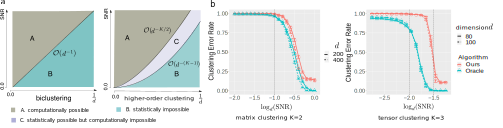
\includegraphics[width=1\textwidth]{phase-transition.pdf}
\vspace{-.5cm}
\caption{(a) Three SNR regimes of statistical and computational behaviors for the order-$K$ dimensional-$d$ tensor block problems. A statistical-computational gap arises only for tensors of order 3 or greater. (b) Simulation confirmation of the discovered gap.}\label{fig:phase-transition}
\end{figure}

To our knowledge, we are among the first to explore the statistical and computational limits for tensor block model. We conjecture that the threshold $d^{K/2}$ is a necessary SNR condition for polynomial-time label recovery. Figure~\ref{fig:phase-transition}b shows the empirical results based on our simulations. In the matrix case, the polynomial estimate (ours) and statistical optimal rate (oracle) undergo similar SNR phase transitions. In contrast, the order-3 tensor clustering reveals a striking gap between polynomial estimate and oracle estimate. Similar puzzles about statistical-computational gaps have attracted enormous interests in modern, non-convex problems~\cite{ma2015computational,richard2014statistical}. We aim to provide rigorous evidence for the following conjecture:

\mybox[gray!20]{
\begin{open}(Conjecture) There exists no polynomial-time algorithm that exactly recovers the block labels in tensor block model when $\text{SNR}=\tO(d^{-K/2-\varepsilon})$, for any $\varepsilon >0$.
\end{open}
}

\vspace{-.3cm}
\subsection{Preliminary Results and Assessing Mechanisms}
\vspace{-.3cm}
Classical statistical theory often focuses on maximum likelihood estimation (MLE). Unfortunately, MLE requires exponential time complexity and is practically less useful for tensor problems. We are currently investigating an efficient polynomial-time algorithm based on the recent advances in non-convex optimization. We propose to combine spectral initialization and alternating optimization for locating local optimum with desired statistical accuracy (Figure~\ref{fig:app}a). Our preliminary analysis shows that the proposed Algorithm~\ref{alg:B} achieves \emph{exact recovery} of block labels under relaxed assumptions than existing algorithms. 


\begin{algorithm}[http]
\caption{Multiway clustering based on tensor block model}\label{alg:B}
\begin{algorithmic}[1]
\INPUT Data tensor $\tY\in \mathbb{R}^{d\times \cdots \times d}$, clustering size $(r,\ldots,r)$.
\OUTPUT Block mean tensor $\hat \tS\in\mathbb{R}^{r\times \cdots\times r}$, and the membership matrices $\hat \mM_k\in\{0,1\}^{r\times d}$. 
\State Initialize the marginal clustering by higher-order spectral clustering. 
\For{$t=1,2,\ldots$}
\State Update the core tensor $\hat \tS$ using the sample averages within each multi-way block. 
\State Update each membership matrix $\hat \mM_k$ by a small nearest neighbor search over $r$ discrete points. 
\EndFor
\end{algorithmic}
\end{algorithm}

My preliminary results reveal a two-component error in the clustering error bound. 
\begin{thm}[Statistical and computational accuracy]\label{nonconvexity} The output from Algorithm~\ref{alg:B} satisfies
\[
\text{Error at step $(t+1)$}\lesssim \KeepStyleUnderBrace{\sigma^2\exp\left(-{d^{K-1}\over r^{K-1}}\SNR\right)}_{\text{statistical error}} + \KeepStyleUnderBrace{\rho^{t}\ \text{Error at step $0$}}_{\text{computational error}}.,
\]
\end{thm}
\vspace{-.3cm}
where  $\rho\in(0,1)$ is a contradiction parameter independent of problem dimensions, and $t=1, 2, \ldots$ denotes the iteration number in the algorithm. This bound reveals the interesting interplay between the computational and statistical errors, and the result immediate suggests a practical tradeoff between these two aspects. One of my main research goals is to understanding the gap between the algorithm property and statistical optimality, which will in turn offer a useful guide to algorithm designs.

Our experience indicates that parametric tensor models often exhibit the \emph{benign nonconvexity} as shown in Theorem~\ref{nonconvexity} and Figure~\ref{fig:app}a. That is, a well-designed local solution achieves similar statistical accuracy as the global MLE, albeit a highly non-convex optimization algorithm. Examples include tensor SVD~\cite{wang2018learning}, tensor completion~\cite{pmlr-v119-lee20i}, and tensor regression~\cite{han2020optimal}. We plan to explore the optimization landscape for a broader range of problems, including exponential-family tensors, orthogonal decomposable tensors, methods-of-moment tensors, deep tensor neural networks, and tensor-based reinforcement learning. 

\mybox[gray!20]{\begin{open} 
Can we characterize the full class of specially-structured tensors for which efficient, provable algorithms exist?\
\end{open}}

My group will assess our proposed research by empirical performance on real data. Figure~\ref{fig:app}b shows the application of our method to flight route data from OpenFlights database. The values in the depicted matrix represent the connectivity of airports based on our clustering results. We find that US airlines tend to show highly concentrated connections among US, Europe, and Asia airports. In contract, mixture airlines tend to have dense but low connections. This reflects the nature of this cluster consisting of many regional airports around the world. The results demonstrate the applicability and potential of our method.

\begin{figure}[http]
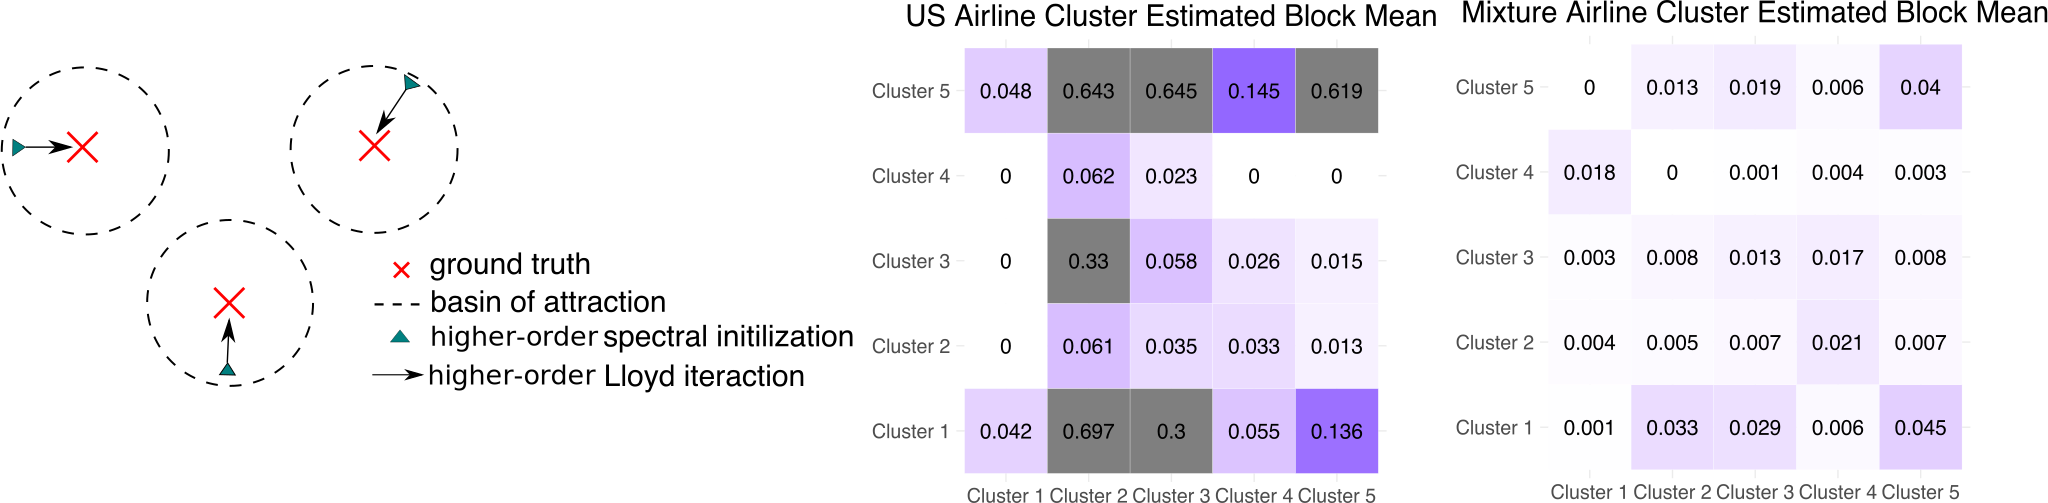
\includegraphics[width=1\textwidth]{demo2.pdf}
\caption{(a) Optimization landscape of tensor block model. (b). Application of higher-order clustering to flight routes data.}\label{fig:app}
\end{figure}

\mybox[gray!20]{
{\bf Significance and transformative concepts:} 
\begin{itemize}[leftmargin=*]
\item Establish statistical learning foundations for unsupervised tensor clustering and dimension reduction. 
\item Design robust and efficient algorithms for large-scale tensor data analysis. 
\item Create data-driven solutions and pipelines for tensor data pattern recognition.
\end{itemize}
 }
 
 \vspace{-.3cm}
\section{AIM 2. Beyond Low-rankness: Nonparametric Estimation for High-rank Tensors}\label{sec:theme2}
\vspace{-.5cm}
Parametric tensor methods often rely on two assumptions:\ (i) a known relationship between observed data and latent low-rank representation, and (ii) a global low-rank structure across all tensor entries. 
\mybox[gray!20]{This section develops a new nonparametric approach to tensor estimation by relaxing these two assumptions. The framework leads to a substantially larger class of signal tensor models than previously possible. }

\vspace{-.3cm}
\subsection{Motivation}\label{sec:intro}
\vspace{-.3cm}
While low-rank methods have shown great success in theory, tensors in applications often violate the parametric form in the model. We provide two examples to illustrate the limitation of classical models.

The first example reveals the sensitivity of tensor rank to order-preserving transformations (Figure~\ref{fig:example}a). Let $\tZ \in \mathbb{R}^{30\times 30\times 30}$ be an order-3 tensor with tensor $\text{rank}(\tZ)=3$. Suppose a monotonic transformation $f(z)=(1+\exp(-cz))^{-1}$ is applied to $\tZ$ entrywise, and we let the signal $\Theta$ be the tensor after transformation. Figure~\ref{fig:example}a plots the numerical rank of $\Theta$ versus $c$. As we see, the rank increases rapidly with $c$, rending traditional low-rank tensor methods ineffective in the presence of mild order-preserving nonlinearities. In many applications, the tensor of interest often undergoes unknown transformation prior to measurements. The sensitivity to transformation makes the parametric model less desirable in practice. 

\begin{figure}[h]
\centering
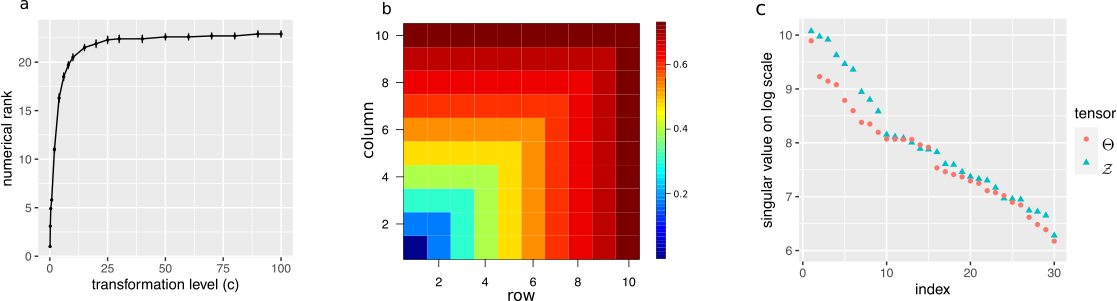
\includegraphics[width=0.9\textwidth]{low_rank.pdf}
\caption{High-rank tensor examples. (a) Numerical rank of tensor $g(\tZ)$ versus $c$ in the transformation. (b) Heatmap of a full-rank matrix $\Theta\in\mathbb{R}^{d\times d}$ with $(i,j)$-th entry equal to $\log(1+\log(i,j))$. (c) Top $d = 30$ tensor singular values in the second example. }\label{fig:example}
\vspace{-.2cm}
\end{figure}

The second example demonstrates the inadequacy of classical low-rankness in representing special structures (Figure~\ref{fig:example}b-c). Here we consider the signal tensor of the form $\Theta=\log(1+\tZ)$, where $\tZ\in\mathbb{R}^{d\times d\times d}$ is an order-3 tensor with entries $\tZ(i,j,k)=d^{-1}\max(i,j,k)$ for $i,j,k\in\{1,\ldots,d\}$. The matrix analogy of $\Theta$ was studied in graphon analysis~\cite{chan2014consistent}; see Figure~\ref{fig:example}b for an illustration. In this case, neither $\Theta$ nor $\tZ$ is low-rank; in fact, Figure~\ref{fig:example}c shows that the rank is no smaller than the dimension $d$. Again, classical low-rank models fail to address this type of tensor structure. 

These examples reveal the inadequacy of the conventional low-rank model in capturing important yet complex tensor structure. The observation has motivated us to develop a flexible class of nonparametric tensor models for estimating nonlinear, local, and possibly high-rank effects. Our goal is to accurately estimate $\Theta$ from the incomplete, noisy observation of $\tY$. In particular, we focus on the following two problems:
\mybox[gray!20]{
\begin{open}
\begin{itemize}[wide]\hfill
\item How to estimate $\Theta$ under a wide range of structures, including both low-rankness and high-rankness?
\item How many observed tensor entries do we need to consistently estimate the signal $\Theta$?
\end{itemize}
\end{open}
}

  \vspace{-.3cm}
\subsection{Proposed Agenda: Nonparametric Sign Representable Tensor Models}
  \vspace{-.3cm}
We plan to develop new tools to address aforementioned challenges. In the earlier two examples, the high-rankness in the signal $\Theta$ makes the estimation challenging. The key crux is to design a new notion of nonparametric complexity that incorporates both low and high-rank tensors. Let us examine the sign of the $\pi$-shifted signal tensor $\sign(\Theta-\pi)$ for a given $\pi\in\mathbb{R}$. Here the operation $\sign(\cdot)$ converts a real-valued tensor to an $\{-1,1\}$-valued tensor in an entrywise fashion. It turns out that, the sign tensors have the same sign patterns as low-rank tensors. Indeed, the signal tensor in the first example has the same sign pattern as a rank-$4$ tensor, since $\sign(\Theta-\pi)=\sign(\tZ-f^{-1}(\pi))$. The signal tensor in the second example has the same sign pattern as a rank-2 tensor, since $\sign(\Theta(i,j,k)-\pi)=\sign(\max(i,j,k)-d(e^{\pi}-1))$.

The above observation suggests a general framework to estimate both low- and high-rank signal tensors. Figure~\ref{fig:demo} illustrates the main idea of our method. Suppose we aim to estimate a signal tensor $\Theta\in[-1,1]^{d\times\cdots\times d}$ from a data tensor observation $\tY=\Theta+\tE$ contaminated by a noise $\tE$ with i.i.d.\ sub-Gaussian entries. We develop a nonparametric estimate $\hat \Theta$ by averaging over the series of de-noised sign tensors
\begin{equation}\label{eq:nonparametric}
\hat \Theta = {1\over 2H+1}\sum_{\pi \in \tH} \sign(\hat \tZ_\pi), \quad \text{where}\ \hat \tZ_\pi=\argmin_{\text{low rank tensor $\tZ$}} \text{Weighted-Loss}(\sign(\tZ), \sign (\tY-\pi)).
\end{equation}
Here $\sign(\hat \tZ_\pi)$ is the de-noised sign tensor estimated at a series of $\pi\in \tH=\{\small-1,\ldots,$ $-{1/H},0, {1/H},\ldots,1\}$, $H\in\mathbb{N}_{+}$ is a pre-specified precision level, and Weighted-Loss$(\cdot, \cdot)$ is a classification objective that assesses the total sign mismatches, with entrywise weights, between two tensor arguments. \begin{figure}[http]
\centerline{\includegraphics[width=1\textwidth]{demo_sign.pdf}}
\caption{Illustration of our nonparametric methods based on based on Example~\ref{eq:example} in Section~\ref{sec:model}. (a): a noisy, incomplete tensor input. (b)-(c): Estimation of sign tensor series $\sign(\Theta-\pi)$ for $\pi\in  \{-1,\ldots,-{1/ H},0,{1/H},\ldots,1\}$. (d): recovered signal $\hat \Theta$.
}\label{fig:demo}
\vspace{-.4cm}
\end{figure}

Our approach is built on the nonparametric representation of signal tensors. Surprisingly, a careful aggregation of dichotomized data not only preserves all information in the original signals, but also brings the accuracy and flexibility over classical low-rank models. The sign representation is guaranteed to recover both low- and high-rank signals. In addition, a total of $H=\text{poly}(d)$ base algorithms suffice to recover $\Theta$ under the considered model.  The method therefore enjoys both statistical and computational efficiency. 

  \vspace{-.3cm}
\subsection{Preliminary Results}\label{sec:model}
  \vspace{-.3cm}
Our future work will formulate the above intuition into a general nonparametric tensor framework. We plan to investigate a rich nonparametric family based on what we coin as the ``sign-rank'' of a tensor. 
\begin{defn}[Sign representable tensors] 
The sign-rank of a tensor $\Theta$ is defined by the minimal rank among all tensors that have the same sign pattern as $\Theta$; i.e., $\text{srank}(\Theta)= \min \{\rank(\Theta')\colon  \sign(\Theta')=\sign(\Theta)\}$. We use $\caliP(r)=\{\Theta\colon \max_{\pi\in[-1,1]}\srank(\Theta-\pi)\leq r\}$ to denote the $r$-sign representable tensor family.
\end{defn}

 \begin{figure}[http]
 \centering
 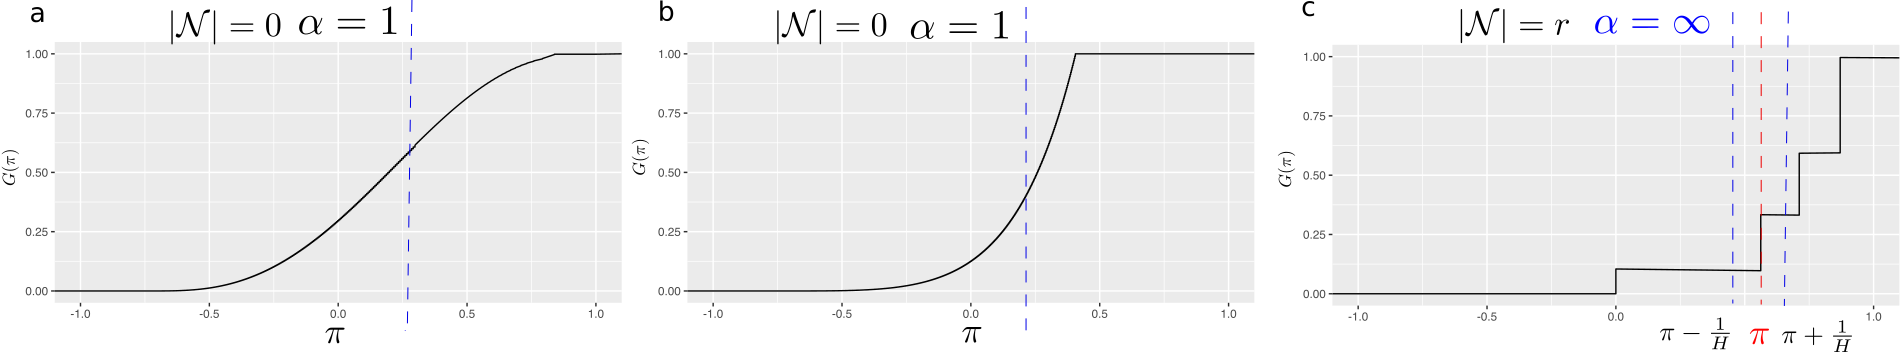
\includegraphics[width = .8\textwidth]{cdf_new.pdf}
 \vspace{-.2cm}
 \caption{(a)-(b) Functions $G(\pi)$ with local H\"older smoothness index $\alpha = 1$; (c) $G(\pi)$ with $\alpha =\infty$ at most $\pi$ (in blue), except for a total number of $|\tN| = r$ jump points (in red). Here $|\tN|$ denotes the number of jump points in $G$.}\label{fig:cdf}
\vspace{-.2cm}
 \end{figure}
 
We characterize the statistical hardness of the estimation problem using $G(\pi)=\mathbb{P}_{\omega\in\Pi}(\Theta(\omega)\leq \pi)$, the cumulative distribution function (CDF) of tensor entries under sampling distribution $\Pi$ over index $\omega\in [d]^K$. See Figure~\ref{fig:cdf} for three examples of $G(\pi)$ with various smoothness behaviors. 
  
 \begin{thm}[L\underline{W}, on-going work] 
 Suppose $\Theta\in\caliP(r)$ is an $\alpha$-smooth tensor with bounded number of jump points. Let $\Omega\subset[d]^K$ denote the index set of observed entries, and assume the entries $\omega$ in $\Omega$ are i.i.d.\ draws with replacement from the full index set using sampling distribution $\Pi$. The global optimizer in~\eqref{eq:nonparametric} based on our method (Figure~\ref{fig:demo}) obeys the following accuracy guarantees.
 \begin{enumerate}[wide]
\item[] (a) (Tensor denoising) For all precision levels $H\in\mathbb{N}_{+}$, with high probability,
{\small \begin{align}\label{eq:bound2}
\mathbb{E}_{\omega\sim \Pi}|\hat \Theta- \Theta|&\lesssim \underbrace{\left({d r\over |\Omega|}\right)^{\alpha\over\alpha+2}}_{\text{Error inherited from sign estimation}}+\underbrace{{1\over H}}_{\text{Bias}}+\underbrace{{Hd r \over |\Omega|}}_{\text{Variance}}\lesssim \left( dr\over|\Omega|\right)^{\min\left({\frac{\alpha}{\alpha+2},\frac{1}{2}}\right)},
\end{align}
}
where the last inequality is obtained by setting $H\asymp|\Omega|/dr$. 
\item[] (b) (Tensor completion). Suppose $\alpha\neq 0$. Then, with high probability, the minimal sample requirement for consistent tensor completion is $\tilde\tO (dr)$, where $\tilde\tO(\cdot)$ hides the logarithmic factors.
    \end{enumerate}
    \end{thm}
    
Our preliminary investigation shows that the $r$-sign representable tensor family is a general model that incorporates most existing tensor models including low-rank tensors, single index models, logistic tensor models, and structured tensors with repeating entries. Table~\ref{compare} shows the outperformance of our estimation accuracy compared to previous methods. 

%\begin{example}[CP/Tucker low-rank model] The CP and Tucker low-rank tensors are the two most popular tensor models~\cite{kolda2009tensor}. Every CP rank-$r$ tensor $\Theta$ belongs to the sign representable family; i.e., $\Theta\in\caliP(r+1)$ (the constant $1$ is due to intercept effects). Similar results hold for Tucker low-rank tensors $\Theta\in\caliP(r+1)$, where $r=\prod_kr_k$ with $r_k$ being the $k$-th mode Tucker rank of $\Theta$.  
%\end{example} 
\begin{example}[Tensor block model] Tensor block model~\cite{wang2019multiway,chi2020provable} assumes a checkerboard structure among tensor entries under marginal index permutation. The signal tensor $\Theta$ takes at most $r$ distinct values, where $r$ is the total number of multiway blocks. Our model incorporates tensor block model in that $\Theta \in \caliP(r)$. 
\end{example}
\begin{example}[Generalized linear model] Logistic tensor model~\cite{wang2018learning} assumes a binary tensor $\tY$ with mean $\Theta=\text{logit}(\tZ)$, where $\tZ$ is a latent low-rank tensor. The mean tensor $\Theta$ itself if often high-rank (see Figure~\ref{fig:example}a); however we find that $\Theta$ has low complexity based on our sign-rank notion. Same results hold for general exponential-family models with a (known) link function~\cite{hong2020generalized}. 
\end{example}

\begin{example}[Single index model] Single index model is a flexible semiparametric model proposed in economics~\cite{robinson1988root} and high-dimensional statistics~\cite{balabdaoui2019least,ganti2015matrix}. The single index model assumes the existence of a (unknown) monotonic function $g\colon \mathbb{R}\to \mathbb{R}$ such that $g(\Theta)$ has rank $r$. We see that $\Theta$ belongs to the sign representable family; i.e., $\Theta\in \caliP(r+1)$. 
\end{example}

\begin{example}[Structured tensors with repeating entries]\label{eq:example} Here we revisit the model introduced in Figure~\ref{fig:example}b. We find that $\Theta \in \caliP(2)$, because the sign tensor $\sign(\Theta-\pi)$ with an arbitrary $\pi\in(0,\ \log 2)$ is a block tensor with at most two blocks (see Figure~\ref{fig:demo}c). 
%Similar results extend to structured tensors with entries $\Theta(i,j, k)=g(\max(i,j,k))$, where $g(\cdot)$ is a polynomial of degree $r$. In this case, $\Theta$ is a high-rank tensor with at most $d$ distinct entries but we have $\Theta\in \caliP(2r)$. 
\end{example}

   
 
 \begin{table}[http]
 \vspace{-.2cm}
 \resizebox{\columnwidth}{!}{
\begin{tabular}{ccl}
Model & Our rate (power of $d$) & Previous results\\
\hline
Tensor block model &$-(K-1)/2$& $\alpha = \infty$; agrees with the minimax rate~\cite{wang2019multiway}.\\
\hline
Generalized linear model &$-(K-1)/3$&  $\alpha=1$;  close to parametric rate~\cite{pmlr-v119-lee20i}.\\ 
\hline
\multirow{2}{*}{Single index model}&\multirow{2}{*}{$-(K-1)/3$}& $\alpha =1$; conjecture to be optimal; our rate in matrix \\
&& case $d^{-1/3}$ improves previous result $d^{-1/4}$~\cite{ganti2015matrix}.\\
\hline
 \multirow{2}{*}{Nonparametric tensor model} & \multirow{2}{*}{$-(K-1)\min({\alpha\over\alpha+2}\wedge {1\over 2} )$}& \multirow{2}{*}{faster rate as smoothness index $\alpha$ increases.} \\&&\\
\hline
\end{tabular}
}
\vspace{-.3cm}
\caption{Comparison of statistical convergence rate between our nonparametric tensor models and previous methods.}\label{compare}
  \vspace{-.3cm}
\end{table}

The current theoretical guarantees we obtain are for the global optimizer. The proposed agenda will focus on characterization of local optimizers, or relatedly, the computational-statistical trade-off for nonparametric tensor estimation. Our extensive experience on tensor related work has shown that tensors sought in applications often possess special structures. These properties provide solutions to address global optimality issues that are impossible in general cases. In a wide range of non-convex problems, all saddle points are strict and all local minima are global minima. My group is actively exploring the interplay between optimization error and statistical accuracy in nonparametric tensor problems. The proposed approach will revolutionize the tensor problems including, but not limited to, tensor SVD, tensor completion, tensor decomposition, and tensor regression.
\mybox[gray!20]{
\begin{open}
\begin{itemize}[wide]\hfill
\item 
What is the minimax optimal statistical rate for nonparametric tensor estimation? 
\item Can we develop polynomial-time algorithms to achieve the optimal statistical rate?
\end{itemize}
\end{open}
}

  \vspace{-.3cm}
\subsection{Assessing Mechanisms}
  \vspace{-.3cm}
We plan to assess the success of our approach using two tensor datasets, the MRN-114 human brain connectivity data~\cite{wang2017bayesian}, and NIPS data~\cite{globerson2007euclidean}. The brain dataset records the structural connectivity among 68 brain regions for 114 individuals along with their Intelligence Quotient (IQ) scores. The NIPS dataset consists of word occurrence counts in papers published from 1987 to 2003. The resulting dataset is an order-3 tensor with entry representing the log counts of words by authors across years. 

Table~\ref{tab:data} and Figure~\ref{fig:signal} show the preliminary data analysis on the two data applications. Table~\ref{tab:data} compares the prediction accuracy of different methods. Reported prediction errors are averaged over five runs of cross-validation, with 20\% entries for testing and 80\% for training. Our method substantially outperforms the low-rank CP method for every configuration under consideration. Figure~\ref{fig:signal}a plots the top brain connections related to IQ scores are mostly inter-hemisphere edges, consistent with recent research on brain connectivity~\cite{wang2017bayesian}. Figure~\ref{fig:signal}b illustrates the results from NIPS data, where we plot the entries in $\hat \Theta$ corresponding to top authors and most frequent words. The identified pattern agrees with active topics in the NIPS publication. Among the top words are \emph{neural} (marginal mean = 1.95), \emph{learning} (1.48), and \emph{network} (1.21), whereas top authors are \emph{T.\ Sejnowski} (1.18), \emph{B.~Scholkopf} (1.17), \emph{M.\ Jordan} (1.11), and \emph{G.\ Hinton} (1.06). The detected pattern and achieved accuracy demonstrate the applicability of our method.

\vspace{-.1cm}
\begin{minipage}[c]{0.4\textwidth}
\resizebox{1\textwidth}{!}{
\def\arraystretch{1.5}
\begin{tabular}{cccc}
\Xhline{2\arrayrulewidth}
\multicolumn{4}{c}{MRN-114 brain connectivity dataset}\\
\Xhline{2\arrayrulewidth}
Method                    & $r=6$ &  $r=9$&$r=12$\\
\hline
{\bf Nonparametric (Ours)}  & ${\bf 0.14}(0.001)$ &  ${\bf 0.12}(0.001)$&${\bf 0.12}(0.001)$\\
CPT  & $0.23(0.006)$&$0.22(0.004)$&$0.21(0.006)$\\
 \Xhline{2\arrayrulewidth}
\multicolumn{4}{c}{NIPS word occurrence dataset}\\
 \Xhline{2\arrayrulewidth}
Method                    & $r=6$& $r=9$&$r=12$\\
\hline
{\bf Nonparametric (Ours)}  & ${\bf 0.16}(0.002)$& ${\bf 0.15}(0.001)$&${\bf 0.14}(0.001)$\\
CPT &$0.20(0.007)$&$0.19(0.007)$&$0.17(0.007)$\\
\hline
\end{tabular}
}
\captionof{table}{Prediction comparison between our method ($H=20$) and low-rank CP method (CPT) in the two data applications. Standard errors are in parenthesis.}\label{tab:data}
\end{minipage}
\hspace{.4cm}
 \begin{minipage}[c]{0.55\textwidth}
 \centering
\includegraphics[width=.4\textwidth]{brainIQ.pdf}
\includegraphics[width=.5\textwidth]{signal.pdf}
\vspace{-.3cm}
\captionof{figure}{(a) top IQ-associated edges in the brain connectivity data. \\
(b) top (authors, words, year) triplets in the NIPS data. }\label{fig:signal}
 \end{minipage}
 
 
\mybox[gray!20]{{\bf Significance and transformative concepts:} 
\begin{itemize}[leftmargin=*]
\item Develop efficient nonparametric prediction tools for tensor classification, tensor regression, and deep tensor neural network, in the presence of computational constraints.
\item Improve efficiency in scientific discovery using powerful multimodal brain data connectivity analyses. 
\item Build data-driven prototypes that integrate tensor data learning into the data-to-decision process. 
\end{itemize}
}

\vspace{-.3cm}
\section{AIM 3: Predictive Tensor Models with Auxiliary Information}\label{sec:theme3}
\vspace{-.5cm}
Tensor datasets are often collected together with additional auxiliary features in modern scientific and engineering studies. In neuroimaging analysis, brain connectivity networks are collected from a sample of individuals, accompanied by individual characteristics such as age, gender, and diseases status (see Figure~\ref{fig:intro1}a). In social network analysis, connectivity strengths between individual pairs are collected, with auxiliary information such as people’s demographic information and friendship types available. In both examples, scientists are interested in learning the relationship between tensor data and auxiliary features. These seemingly different scenarios pose a common yet challenging problem for predictive tensor data modeling. 

\begin{figure*}[http]
\begin{center}
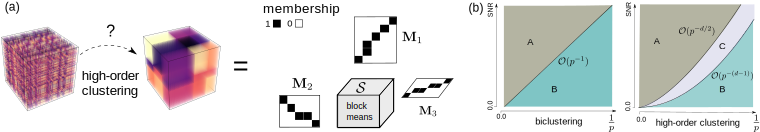
\includegraphics[width=16cm]{demo.pdf}
\end{center}
\caption{Examples of predictive tensor models with auxiliary information. (a) Network regression with auxiliary information. (b) Spatial-temporal growth data represented as an order-3 tensor $\tY$, where feature matrices $\mX_k$ are on each of the three modes.}\label{fig:intro1}
\vspace{-.2cm}
\end{figure*}

  \vspace{-.2cm}
\subsection{Three Motivating Examples}
  \vspace{-.3cm}
We give three concrete examples to highlight the applicability of predictive tensor models.
 \begin{example}[Dyadic data with node attributes]\label{ex:3} Dyadic dataset consists of measurements on pairs of objects. Common examples include graphs and networks. Let $\tG=(V,E)$ denote a graph, where $V=[d]$ is the node set of the graph, and $E\subset V\times V$ is the edge set. Suppose that we also observe feature $\mx_i\in\mathbb{R}^p$ associated to each node $i\in V$. A probabilistic model on the graph $\tG=(V,E)$ can be described by matrix regression. The edge connects the two vertices $i$ and $j$ independently of other pairs, and the probability of connection is modeled as
\begin{equation}\label{eq:edge}
\mathbb{P}\left((i,j)\in E|\mx_i,\mx_j \right)=\text{logistic}(\langle \mB,\ \mx^T_i\mx_j\rangle),
 \end{equation}
 where $\mB\in\mathbb{R}^{p\times p}$ is an unknown parameter matrix of interest. The dyadic data is a predictive matrix model that uses matrix coefficient $\mB$ for structure learning and edge prediction. 
  \end{example}
  
\begin{example}[Network regression model]\label{example:brain}
Network response model~\cite{zhang2018network} is recently developed for neuroimanig analysis. The goal is to study the relationship between brain network connectivity patterns and individual's features. Suppose we have a sample of $n$ observations, $\{(\mY_i, \mx_i)\colon i=1,\ldots,n\}$, where for each individual $i\in[n]$, $\mY_i\in\{0,1\}^{d\times d}$ is the symmetric adjacency matrix whose entries indicate presences/absences of connectivities between $d$ brain nodes, and $\mx_i\in\mathbb{R}^p$ is the individual's feature such as age, gender, cognition score, etc. The network regression models takes the form
\[
\mathbb{E}(\mY_i |\mx_i)=\text{logistic}(\tB\times_3\mx_i), \quad \text{or more generally}  \quad \mathbb{E}(\mY_i |\mx_i)=f(\tB\times_3\mx_i), 
\]
where $\tB\in\mathbb{R}^{d\times d\times n}$ is the unknown parameter tensor of interest, and $f\colon\mathbb{R}\to\mathbb{R}$ is a possibly unknown function. The network regression (Figure~\ref{fig:intro1}b) is a predictive tensor model that uses tensor coefficient $\tB$ for structure learning and connectivity prediction.  
\end{example}
 
\begin{example}[Spatio-temporal growth model]\label{ex:1}
The growth curve model~\cite{gabriel1998generalised} was originally proposed as a bilinear model for matrix data, and we adopt its higher-order extension here. Let $\tY=\entry{y_{ijk}}\in\mathbb{R}^{d \times m\times n}$ denote the pH measurements of $d$ lakes at $m$ levels of depth and for $n$ time points. %Suppose the sampled lakes belong to $q$ types, with $p$ lakes in each type. Let $\{\ell_j\}_{j\in[m]}$ denote the sampled depth levels and $\{t_k\}_{k\in[n]}$ the time points. 
Assume that the expected pH trend is polynomial in depth and in time. Then, the multilinear growth curve model is represented as
\begin{equation}\label{eq:time}
\mathbb{E}(\tY|\mX_1,\mX_2,\mX_3)=\tB\times_1\mX_1\times_2 \mX_2\times_3 \mX_3,
\vspace{-.15cm}
\end{equation}
where $\mX_1, \mX_2, \mX_3$
%=\text{blockdiag}\{\mathbf{1}_p,\ldots,\mathbf{1}_p\}\in \{0,1\}^{d\times q}$ is the design matrix for lake types, and $\mX_2, \mX_3$
%\[
%\mX_2=
%\begin{pmatrix}
%1 & \ell_1&\cdots &\ell^{r}_1\\
%1 & \ell_2&\cdots &\ell^{r}_2\\
%\vdots &\vdots&\ddots&\vdots\\
%1&\ell_{m}&\cdots&\ell^{r}_{m}
%\end{pmatrix},\quad
%\mX_3=
%\begin{pmatrix}
%1 & t_1&\cdots &t^{s}_1\\
%1 & t_2&\cdots &t^{s}_2\\
%\vdots &\vdots&\ddots&\vdots\\
%1&t_{n}&\cdots&t^{s}_{n}
%\end{pmatrix}
%\]
are the design matrices for lake types, spatial effects, and temporal effects, respectively, $\tB\in\mathbb{R}^{d_1\times d_2\times d_3}$ is the unknown parameter tensor of interest. The spatial-temporal model (Figure~\ref{fig:intro1}a) belongs to the predictive tensor model, with the tensor $\tB$ serving the role of joint structure learning and response prediction. 
\end{example}
\mybox[gray!20]{{\bf Significance and transformative concepts:} 
\begin{itemize}[leftmargin=*]
\item Develop powerful predictive tensor models for joint structure estimation and function learning. 
\item Address tensor data mining challenges with interpretable inference and uncertainty quantification. 
\item Foster interdisciplinary research that integrates methodological developments and domain sciences.
\end{itemize}
}
  \vspace{-.3cm}
\subsection{Proposed Agenda: Tensor Neural Network Models}
  \vspace{-.3cm}
The proposed project focuses on developing a general framework for tensor learning and prediction with auxiliary information. The aforementioned examples represent three different forms of predictive tensor regression models, i.e., whether tensor is treated as predictors (Example~\ref{ex:3}), as responses (Example~\ref{example:brain}), or both (Example~\ref{ex:1}). Here we outline the research direction for the first setting; the generalization to the other two are similar. 

We propose to formulate the predictive task as learning the regression function between tensor predictor $\tX\in\mathbb{R}^{d_1\cdots \times d_K}$ and the scalar response $Y\in\mathbb{R}$. Based on the i.i.d.\ training set $(\tX_i, Y_i)_{i=1,\ldots,n}$, we aim to estimate the conditional mean of $Y$ as a function of $\tX$ based on the tensor neural network model
\begin{equation}\label{eq:NN}
Y|\tX=f(\tX)+\varepsilon, \quad \text{where}\quad f(\tX)=\sum_{h=1}^H v_h \sigma(\langle \tB_h, \tX\rangle-\pi_h),
\end{equation}
where $\varepsilon$ is a zero-mean sub-Gaussian noise, $\sigma\colon \mathbb{R}\to\mathbb{R}$ is a pre-specified activation function, $\tX\mapsto\langle \tB_h, \tX \rangle$ is the trace effect with an unknown parameter tensor $\tB_h\in\mathbb{R}^{d_1\times \cdots \times d_K}$, $v_h, \pi_h \in\mathbb{R}$ are unknown scalar parameters, and $h=1,\ldots,H$ is the index in function basis representation. The activation function is often nonlinear so that $f$ is also nonlinear in parameter $\tB_h$. Figure~\ref{fig:intro1} illustrates our model with activation function $\sigma(z)=\sign(z)$. Other common activation functions are Rectified Linear Unit (ReLU) $\sigma(z)=z_{+}$ and logistic $\sigma(z)=(1+\exp(-z))^{-1}$. The model~\eqref{eq:NN} extends the multivariate two-layer neural network to tensor data, so we refer it to as ``tensor neural network'' (see Figure~\ref{fig:intro1}).  


\begin{figure}[http]
\begin{center}
\includegraphics[width=.9\textwidth]{ASSIST.pdf}
\caption{Proposed tensor neural network model for predictive tensor learning tasks.}\label{fig:proposal}
\vspace{-.3cm}
\end{center}
\end{figure}


Our proposed tensor neutral network (Figure~\ref{fig:intro1}) blends the power of neural network and structure learning in order to take the best out of both worlds. Learning parameter tensors $\tB_h$ in~\eqref{eq:NN} is challenging because of the extremely high dimensionality in the tensor space and functional space. The PI's previous extensive experience on tensor related work has shown that tensors sought in applications often possess special structures, such as (nearly) low-rankness, sparsity, non-negativity, and smoothness. We will leverage the formalisms of \emph{intrinsic dimension} to impose suitable structure models on $\tB_h$. The structure-revealing model effectively mitigates the curse of high dimensionality. We will further develop multi-layer tensor neural network that incorporates practical constraints in domain applications, such as incomplete observation with missing labels, corrupted distributions, and computation with time and memory constraints.

\mybox[gray!20]{{\bf Breaking previous limits:} \hfill 
\begin{itemize}[wide]
\item Do higher-order tensors require a completely new modeling paradigm compared to traditional data? 
\item How to develop robust, adaptive estimates that achieve both statical and computational efficiency? 
\end{itemize}
Solving these questions will revolutionize the tensor learning research by bridging theory and practice.}



\vspace{-.3cm}
\section{Integration of Education and Research}\label{sec:impact}
\vspace{-.5cm}
The project will create deliverables in three aspects: {\bf research}, {\bf education}, and {\bf social good}. Figure~\ref{fig:proposal} summarizes the planned milestones and deliverables; details will be described in the next paragraph. My plan consists of a range of activities aimed at increasing understanding, awareness, and participation in data science, integrated with the research and teaching agenda in this proposal. 

\begin{figure}[!ht]
\begin{center}
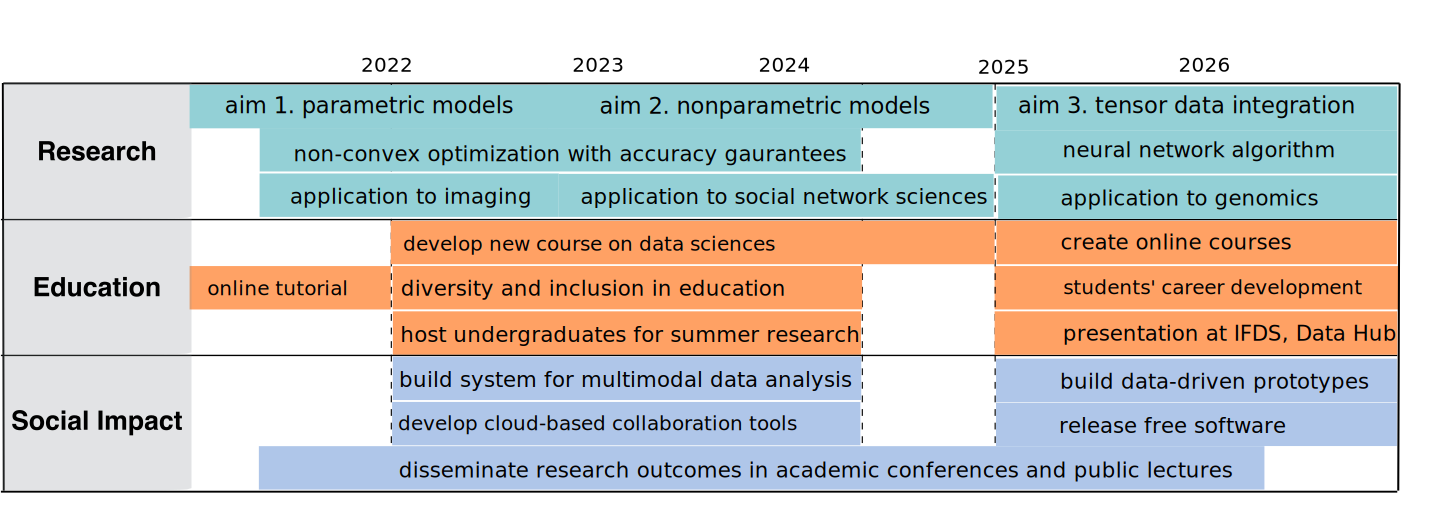
\includegraphics[width=.98\textwidth]{milestone.pdf}
\caption{Planned deliverables and milestones in my proposal.}\label{fig:proposal}
\end{center}
\end{figure}

  \vspace{-.42cm}
\subsection{Education and Diversity}
  \vspace{-.3cm}
I am one of the few female faculty members in my home department. As a young academic, I have been committed to promoting diversity, equity, and inclusion throughout all facets of my career -- in teaching, education, and research. I am currently starting my fourth year in the tenure track, and I have successfully mentored a number of female undergraduate students -- two of which are embarking on their PhD studies at top US universities this fall. Female students are traditionally underrepresented in my filed, and I have been striving to motivate more women in my research. My experience of recruiting underrepresented students has attracted social media coverage~\cite{wang11}. With the support of CAREER research grant, I will extend this effort to a larger student body by creating unique research-training experience to more diverse undergraduates. 

I plan to create a new course on \emph{fairness in data science} in both traditional and online formats. This course will introduce students to address bias and fairness when deploying data science system, and will be closely tied with social science and scientific domains. The pedagogical tools will draw on my rich teaching experience and recent success as the Madison Teaching and Learning Excellence (MTLE) Fellow~\cite{wang12}. I will apply active learning techniques in my class. Statistics, as a discipline, transforms ``data'' into ``information''. However data are not just numbers; they are numbers with social, economical, and cultural contexts. My new course will promote critical thinking skills and develop equitable access for underrepresented groups. The personnel constitution in our education environment is becoming increasingly diverse, reflecting the variety witnessed in our broader society. Diversity can be measured across many dimensions -- gender, ethnicity, origin, age, etc. Nevertheless, diversity is not limited to these visible physical differences; diversity also consists of difference in each student’s personality (introvert vs.\ extravert), learning skills, social status, emotional development, and every aspect that distinguishes one individual from another. I believe that every student is unique in their own way, and I will create an open, inclusive education environment that prepares students to become better professionals in the larger, dynamic society.

\vspace{-.3cm}
\subsection{Nurturing the Next Generation of Statisticians}
\vspace{-.3cm}
The educational plan to establish a unique research-training experience and broaden participation in STEM will be well integrated with the research agenda. The outreach activities are targeted at several different populations: PhD students, undergraduate students, minority students, visiting international students, and AP students at Madison West High School. I have and will continue to leverage my professional affiliations in Women in Probability, Women in Machine Learning, and Institute for Foundations of Data Science (IFDS), to engage a diverse pool of students into STEM fields. 

I will establish my group as a unique center for tightly integrated training in two key components: disciplinary expertise and collaborative skills. The multi-disciplinary nature of my publication record, the current spread of projects in my group, and the details of the proposed research make this goal very realistic. Beyond research goals, my mentoring will provide skills, knowledge, and experience to prepare every student to achieve their highest potential. Specific agenda includes:
\begin{itemize}[wide,labelwidth=!, labelindent=0pt,itemsep=0ex,parsep=0ex,topsep=-3pt]
\item Interaction with the PI:
\begin{itemize}
\item The orientation meeting will involve in-depth conversations between the PI and the students to establish the common goals. Key topics include the career development, amount of independence the students require, work habits, research productivity expectation, and data/code ethnicity.
\item Have regular one-on-one meeting with the students to review progress, provide feedback, exchange new techniques, help with publication and fellowship application.
\end{itemize}
\item Individual career guidance:
\begin{itemize}
\item Provide supports to students on personal branding techniques including resume writing, interview preparation, faculty-job searching, and career path outside the academia.
\item Train the students into the new generation of statisticians that have strong skills in quantitative reasoning and problem solving to address large-scale data problems now readily available.
\end{itemize}
\item Outreach activity:
\begin{itemize}
\item Partner with the Data Science Hub and the Division of Diversity, Equality \& Education Achievement (DDEEA) program at UW-Madison to broaden participation in STEM. 
\item Provide students the collaborative skills to make independent, insightful contributions to the society.
\item Sponsor students for at least two conferences or meetings each year (travel cost included in the budget), with the goal to build up students' visibility and emotional ownership for their career development.   

\end{itemize}
\end{itemize}

  \vspace{-.3cm}
\subsection{Broader Impacts}
  \vspace{-.3cm}
The mission of this proposal is to foster an interdisciplinary research team in a way that benefits fellow scientists, academia, and larger society. The proposed research will engage a diverse pool of underrepresented students into STEM, and establish an inclusive environment where every student can success in their own future careers. The PI will organize a series of tutorials on tensor data analytics, with the theme to encourage interdisciplinary collaborations. The PI's ongoing collaborations include research groups at University of Chicago, University of California-Berkeley, and Chan Zuckerberg Biohub. Further collaboration will continue through the NSF-funded TRIPODS (+X) Institute for which the PI is affiliated faculty. Research outputs will be disseminated through publications and software packages with detailed documentation. The PI's group have released over 15 open-source packages in R, Matlab, and C++ at Github thus far. These software packages will provide reproducible research that benefits the larger society. 
\newpage
\setcounter{page}{1}

{\def\section*#1{\bf \Large References}
\begin{thebibliography}{9}
\normalsize
\bibitem{wang2019three} {\bf Miaoyan Wang}, Jonathan Fischer, Yun S Song, Three-way clustering of multi-tissue multi-individual gene expression data using semi-nonnegative tensor decomposition, The Annals of Applied Statistics 13 (2019), No. 2, 1103-1127.
\bibitem{wang2018learning} {\bf Miaoyan Wang} and Lexin Li, Learning from binary multiway data: Probabilistic tensor decomposition and its statistical optimality, Journal of Machine Learning Research 154 (2021), 1-38.
\bibitem{wang2019multiway} {\bf Miaoyan Wang} and Yuchen Zeng, Multiway clustering via tensor block models, Advances in Neural Information Processing Systems 33 (2019), 713-723.
\bibitem{wang5}{\bf Miaoyan Wang}, Fabrice Roux, Claudia Bartoli, Carine Huard-Chauveau, Christopher Meyer, Hana Lee, Dominique Roby, Mary Sara McPeek, and Joy Bergelson. Two-way mixed-effects methods for joint association analyses using both host and pathogen genomes, Proceedings of the National Academy of Sciences (direct submission) 115 (2018) No. 24, E5440-E5449. \\
\underline{Top 5\%} attention score among research articles tracked by Altmetric; \underline{Top 11\%} among all papers published in PNAS.
Platform talk \underline{(top 13\%)} at the 2nd Probabilistic Modeling in Genomics, Cold Spring Harbor Laboratory, 

\bibitem{wang7} {\bf Miaoyan Wang} and Yun S. Song. Tensor decomposition via two-mode higher-order SVD (HOSVD), Journal of Machine Learning Research W\&CP 54 (AISTATS track 2017), 614-622.
\bibitem{wang8} {\bf Miaoyan Wang}, Khanh Dao Duc, Jonathan Fischer, and Yun S. Song. Operator Norm inequalities between tensor unfoldings on the partition lattice, Linear Algebra and its Applications 520 (2017), 44-66.
\bibitem{wang9} {\bf Miaoyan Wang}, Johanna Jakobsdottir, Albert V Smith, Mary Sara McPeek. G-STRATEGY: Optimal selection of individuals for sequencing in genetic association studies, \underline{Editor’s Pick} in Genetic Epidemiology 40 (2016), No. 6, 446-60. \\
\underline{2014 Charles J. Epstein Trainee Award} semifinalist (27 predoctoral recipients out of $\sim$550 candidates) from American Society of Human Genetics (ASHG); Platform talk \underline{(top 8\%)} in 2014 ASHG meeting.  \\
\underline{2013 IGES Williams Award} -- finalist (3 predoctoral recipients out of 156 candidates) from International Genetic Epidemiology Society (IGES); Platform talk in 2013 IGES meeting. 
\bibitem{wang3} Jiaxin Hu, Chanwoo Lee and {\bf Miaoyan Wang}. Supervised Tensor Decomposition with interactive side information (2021). arXiv:1910.09499. \\
\underline{2021 Best Student Paper Award} from the Statistical Computing and Graphics Section of American Statistical Association (ASA).
\bibitem{han2020exact} Rungang Han, Yuetian Luo, {\bf Miaoyan Wang}, and Anru R Zhang, Exact clustering in tensor block model: Statistical optimality and computational limit (2021).  arXiv:2012.09996. \\
\underline{2021 Best Student Paper Award} from the Statistical Learning and Data Science Section of the American Statistical Association (ASA).
\bibitem{pmlr-v119-lee20i} Chanwoo Lee and {\bf Miaoyan Wang}, Tensor denoising and completion based on ordinal observations, International Conference on Machine Learning (2020), 5778-5788.
\bibitem{wang4} Jiaxin Hu, Chanwoo Lee, and {\bf Miaoyan Wang}. Learning multiple networks via supervised tensor decomposition, Neural Information Processing Systems 34 (2020), Workshop on Machine Learning and the Physical Sciences. 
\bibitem{wang6} Duo Jiang and {\bf Miaoyan Wang}. Recent developments in statistical methods for GWAS and high-throughput sequencing studies of complex traits, Biostatistics and Epidemiology 2 (2018), No. 1, 132-159.
\bibitem{wang1} Chanwoo Lee and {\bf Miaoyan Wang}. Beyond the signs: nonparametric tensor completion via sign series, Under review by Neural Information Processing Systems 35 (2021). arXiv:2102.00384.
\bibitem{wang2} Chanwoo Lee, Lexin Li, Helen Zhang, and {\bf Miaoyan Wang}. Nonparametric trace regression in high dimensions via sign series representation, Under review by Annals of Statistics (2021).
\bibitem{wang10} B. W. Engelmann, Y. Kim, {\bf Miaoyan Wang}, B. Peters, R. S. Rock, and P. D. Nash. The development and application of a quantitative peptide microarray platform to protein interaction domain specificity space, Molecular and Cellular Proteomics 13 (2014), No. 12, 3647-62.
\bibitem{wang11} {\bf Miaoyan Wang} and Julie Warner, Women in STEM: 5 Thoughtful Ways to Recruit and Retain Them, Course Hero faculty club feature article (2020). https://www.coursehero.com/faculty-club/classroom-tips/miaoyan-wang/. 
\bibitem{wang12} {\bf Miaoyan Wang} and et al. UW-Madison Teaching and Learning Excellence Fellow (2020). https://mtle.wisc.edu/about-us/meet-the-fellows/omicron-cohort/. 
\bibitem{balabdaoui2019least} Fadoua Balabdaoui, C\'ecile Durot, and Hanna Jankowski, Least squares estimation in the monotone single index model, Bernoulli 25 (2019), No. 4B, 3276-3310.
\bibitem{belkin2019reconciling} Mikhail Belkin, Daniel Hsu, Siyuan Ma, and Soumik Mandal, Reconciling modern machine-learning practice and the classical bias–variance trade-off, Proceedings of the National Academy of Sciences 116 (2019), No. 32, 15849-15854.
\bibitem{bruno2011multimodal} Marie-Aur\'elie Bruno, D Fern\'andez-Espejo, Remy Lehembre, Luaba Tshibanda, Audrey Vanhaudenhuyse, Olivia Gosseries, Emilie Lommers, Martino Napolitani, Quentin Noirhomme, M\'elanie Boly, et al., Multimodal neuroimaging in patients with disorders of consciousness showing functional hemispherectomy, Progress in Brain Research 193 (2011), 323-333.
\bibitem{chan2014consistent} Stanley Chan and Edoardo Airoldi, A consistent histogram estimator for exchangeable graph models, International Conference on Machine Learning (2014), 208-216.
\bibitem{chi2020provable} Eric C Chi, Brian J Gaines, Will Wei Sun, Hua Zhou, and Jian Yang, Provable convex co-clustering of tensors, Journal of Machine Learning Research 21 (2020), No. 214, 1-58.
\bibitem{de2000multilinear} Lieven De Lathauwer, Bart De Moor, and Joos Vandewalle, A multilinear singular value decomposition, SIAM Journal on Matrix Analysis and Applications 21 (2000), No. 4, 1253-1278.
\bibitem{faskowitz2018weighted} Joshua Faskowitz, Xiaoran Yan, Xi-Nian Zuo, and Olaf Sporns, Weighted stochastic block models of the human connectome across the life span, Scientific Reports 8 (2018), No. 1, 1-16.
\bibitem{gabriel1998generalised} Gabriel, K. Ruben. Generalized bilinear regression, Biometrika 85 (1998), No. 3, 689-700.
\bibitem{gandy2011tensor}Silvia Gandy, Benjamin Recht, and Isao Yamada, Tensor completion and low-rank tensor recovery via convex optimization, Inverse Problems 27 (2011), No. 2, 025010.
\bibitem{ganti2015matrix}Ravi Sastry Ganti, Laura Balzano, and Rebecca Willett, Matrix completion under monotonic single index models, Advances in Neural Information Processing Systems (2015), 1873-1881.
\bibitem{ge2020optimization}Rong Ge and Tengyu Ma, On the optimization landscape of tensor decompositions, Mathematical Programming (2020), 1-47.
\bibitem{ghadermarzy2018learning}Navid Ghadermarzy, Yaniv Plan, and Ozgur Yilmaz, Learning tensors from partial binary measurements, IEEE Transactions on Signal Processing 67 (2018), No. 1, 29-40.
\bibitem{globerson2007euclidean}Amir Globerson, Gal Chechik, Fernando Pereira, and Naftali Tishby, Euclidean embedding of co-occurrence data, Journal of Machine Learning Research 8 (2007), 2265-2295.
\bibitem{han2020optimal}Rungang Han, Rebecca Willett, and Anru Zhang, An optimal statistical and computational framework for generalized tensor estimation, Annals of Statistics, In press (2020).
\bibitem{hong2020generalized}David Hong, Tamara G Kolda, and Jed A Duersch, Generalized canonical polyadic tensor decomposition, SIAM Review 62 (2020), No. 1, 133-163.
\bibitem{kolda2009tensor}Tamara G Kolda and Brett W Bader, Tensor decompositions and applications, SIAM review 51 (2009), No. 3, 455-500. 
\bibitem{lei2019consistentcommunity}Jing Lei, Kehui Chen, and Kevin Lynch, Consistent community detection in multilayer network data, Biometrika, to appear (2019).
\bibitem{mele2015human}Marta Mel\'e, Pedro G Ferreira, Ferran Reverter, David S DeLuca, Jean Monlong, Michael Sammeth, Taylor R Young, Jakob M Goldmann, Dmitri D Pervouchine, Timothy J Sullivan, The human transcriptome across tissues and individuals, Science 348 (2015), No. 6235, 660-665.
\bibitem{ma2015computational}Zongming Ma and Yihong Wu, Computational barriers in minimax submatrix detection, The Annals of Statistics 43 (2015), No. 3, 1089-1116.
\bibitem{murdoch2019definitions}W James Murdoch, Chandan Singh, Karl Kumbier, Reza Abbasi-Asl, and Bin Yu, Definitions, methods, and applications in interpretable machine learning, Proceedings of the National Academy of Sciences 116 (2019), No. 44, 22071-22080.
\bibitem{pananjady2020isotonic}Ashwin Pananjady and Richard J Samworth, Isotonic regression with unknown permutations: Statistics, computation, and adaptation (2020), arXiv:2009.02609.
\bibitem{richard2014statistical}Emile Richard and Andrea Montanari, A statistical model for tensor PCA, Advances in Neural Information Processing Systems (2014), 2897-2905.
\bibitem{robinson1988root}Peter M Robinson, Root-$n$-consistent semiparametric regression, Econometrica: Journal of the Econometric Society (1988), 931-954.
\bibitem{sun2015provable}Will Wei Sun, Junwei Lu, Han Liu, and Guang Cheng, Provable sparse tensor decomposition, Journal of Royal Statistical Association Society, Series B 79 (2017), No. 3, 899-916.
\bibitem{timpson2018genetic}Nicholas J Timpson, Celia MT Greenwood, Nicole Soranzo, Daniel J Lawson, and J Brent Richards, Genetic architecture: the shape of the genetic contribution to human traits and disease, Nature Reviews Genetics 19 (2018), No. 2, 110.
\bibitem{NEURIPS2020_f9d3a954}Xiang Wang, Chenwei Wu, Jason D Lee, Tengyu Ma, and Rong Ge, Beyond lazy training for over-parameterized tensor decomposition, Advances in Neural Information Processing systems (2020) 21934-21944.
\bibitem{wang2017bayesian}Lu Wang, Daniele Durante, Rex E Jung, and David B Dunson, Bayesian network-response regression, Bioinformatics 33 (2017), No. 12, 1859-1866.
\bibitem{young2018universality}Jean-Gabriel Young, Guillaume St-Onge, Patrick Desrosiers, and Louis J Dub\'e, Universality of the stochastic block model, Physical Review E 98 (2018), No. 3, 032309.
\bibitem{zhou2013tensor}Hua Zhou, Lexin Li, and Hongtu Zhu, Tensor regression with applications in neuroimaging data analysis, Journal of the American Statistical Association 108 (2013), No. 502, 540-552.
\bibitem{zhang2018network}Jingfei Zhang, Will Wei Sun, and Lexin Li, Network response regression for modeling population of networks with covariates (2018), arXiv:1810.03192 .
\bibitem{zhang2018tensor}Anru Zhang and Dong Xia, Tensor SVD: Statistical and computational limits, IEEE Transactions on Information Theory 64 (2018), No. 11, 7311-7338.
\end{thebibliography}
}
\end{document}